\chapter{Generics}
\label{chap:generics}

\fcolorbox{black}[HTML]{E9F0E9}{\parbox{\textwidth}{%
\noindent \textbf{Learning goals}\\
The junior-colleague
\begin{enumerate}[nolistsep]
\item can explain what generics is.
\item can describe type erasure and the consequences of type erasure
\item can use generic classes, methods and interfaces
\item can create generic classes, method and interfaces
\end{enumerate}}}

\begin{summary}
Java Generics provides the ability to write generic code that is independent of a data type. When a developer uses a generic class,  interface,  or method,  he will specify which data type will acutally be used. The Java Collections framework is entirely written generically. The moment you use an ArrayList,  you need to indicate the data type for the elements of your list.
\end{summary}

\section{Before generics}
Java is a strongly typed programming language.  During the compilation of a program, you will be pointed out if you use the wrong data type.

\begin{lstlisting}
Object aReference = new Movie("Brother Bear");
Integer luckyNumber = aReference;
\end{lstlisting}

The second line of code results in a compilation error.

 

When Java was introduced, this datatype check was not implemented in the Java Collections framework. The following code compiles without errors.  As soon as you execute the program, an exception will occur.

\begin{lstlisting}
import java.util.ArrayList;
import java.util.Iterator;

public class BeforeGenerics {

	public static void main(String[] args) {
		ArrayList objecten = new ArrayList();
		objecten.add(1);
		objecten.add(5.4);
		objecten.add(new Movie("Inception"));

		Iterator iterator = objecten.iterator();
		double total = 0;
		while (iterator.hasNext()) {
			total += (Double) iterator.next();
		}
		System.out.println(total);
	}
}
\end{lstlisting}


\begin{verbatim}
Exception in thread "main" java.lang.ClassCastException: class java.lang.Integer 
cannot be cast to class java.lang.Double (java.lang.Integer and java.lang.Double 
are in module java.base of loader 'bootstrap')
	at be.pxl.ja.BeforeGenerics.main(BeforeGenerics.java:24)
\end{verbatim}

Type-safety was introduced in the Java Collections framework since Java 5. 
When you open the java documentation for the class java.util.ArrayList, you will see the generic parameter  $<E>$. 
E is the type-parameter en makes it possible to provide a datatype for the elements of the ArrayList. 

\begin{lstlisting}
/**
 * Resizable-array implementation of the {@code List} interface.  Implements
 * all optional list operations, and permits all elements, including
 * {@code null}. 
 * ...
 * @param <E> the type of elements in this list
 *
 * @author  Josh Bloch
 * @author  Neal Gafter
 * @see     Collection
 * @see     List
 * @see     LinkedList
 * @see     Vector
 * @since   1.2
 */
public class ArrayList<E> extends AbstractList<E>
        implements List<E>, RandomAccess, Cloneable, java.io.Serializable {
        
    transient Object[] elementData;
    
    /**
     * Returns the element at the specified position in this list.
     *
     * @param  index index of the element to return
     * @return the element at the specified position in this list
     * @throws IndexOutOfBoundsException {@inheritDoc}
     */
    public E get(int index) {
        Objects.checkIndex(index, size);
        return elementData(index);
    }
    
    E elementData(int index) {
        return (E) elementData[index];
    }
    
    ...
}
\end{lstlisting}

\begin{lstlisting}
import java.util.ArrayList;
import java.util.Iterator;

public class SinceGenerics {

	public static void main(String[] args) {

		ArrayList<Double> objecten = new ArrayList<>();
		objecten.add((double) 1);
		objecten.add(5.4);
		//objecten.add(new Movie("Inception"));

		Iterator<Double> iterator = objecten.iterator();
		double total = 0;
		while (iterator.hasNext()) {
			total += iterator.next();
		}
		System.out.println(total);
	}
}
\end{lstlisting}

If you were to add a Movie-object to an ArrayList that accepts Double-objects, you get a compile error.

\begin{verbatim}
Error:(16, 30) java: incompatible types: be.pxl.ja.streamingservice.model.Movie 
cannot be converted to java.lang.Double
\end{verbatim}

When calling the constructor of a generic class, we use the diamond operator $<>$. The compiler can infer the datatype of the objects in the ArrayList (this is called type inference).  We don't need to repeat the datatype when calling the constructor and use the diamond operator.


\section{Writing generic classes}

The generic class Duo  contains a pair of objects of the generic datatype T.  The class definition identifies this class as a generic class by using the type parameter T (<T>).  In the Duo class, you can use T as the datatype for fields,  parameters,  and returntype.

\begin{lstlisting}
public class Duo<T> {
	private T first;
	private T second;

	public Duo(T first, T second) {
		this.first = first;
		this.second = second;
	}

	public T getFirst() {
		return first;
	}

	public T getSecond() {
		return second;
	}
}
\end{lstlisting}

At the moment you create objects of the class Duo,  you will indicate which actual datatype the type parameter T should be replaced with.  For a developer, it looks like the type parameter T is replaced by the chosen datatype.


\begin{lstlisting}
public class DifferentDuos {

	public static void main(String[] args) {
		Duo<String> cocktail = new Duo<>("gin", "tonic");
		System.out.println(cocktail.getFirst());
		Duo<Actor> famousDuo = new Duo<>(new Actor("Ben","Stiller"), new Actor("Owen", "Wilson"));
		Duo<Integer> numbers = new Duo<>(5, 12);
	}

}
\end{lstlisting}

\subsection{Naming conventions}

To avoid confusion between actual classes and generic type parameters in Java, it is important to use correct naming conventions. We will always use a single uppercase letter to name a type parameter.   According to the code conventions, you should never use a single uppercase letter as the name for a class; you must always use meaningful class names. Therefore, when you see a single uppercase letter in Java code, you may assume it is a generic parameter.

We adhere to the following guidelines:

\begin{itemize}
\item E – Element (used in the Java Collections Framework)
\item K – Key (used in Map)
\item N – Number
\item T – Type
\item V – Value (used in Map)
\item S,U,V etc. – use when T already in use
\end{itemize}

\section{Generic interfaces}

\subsection{Interface $Comparable<T>$}

The generic interface $Comparable<T>$ makes it possible to compare objects. 

Once a class implements this $Comparable<T>$ interface, you can use methods like Collections.sort(...) to sort a collection containing objects of this class. We call this ordering the natural order of the class.

When a class implements the $Comparable<T>$ interface, you fill in the type parameter T with the class itself. You must implement the method \textit{int compareTo(T e)}. Through the implementation of this method, you can compare any object of the class with another object of the same class. The int compareTo(T e) method returns:
\begin{itemize}
\item 0 if both objects are equal.
\item -1 or a negative number if this is less than the argument.
\item 1 or a positive number if this is greater than the argument.
\end{itemize}

Always try to keep the natural order of a class consistent with the implementation of equals()-method.  So, when e1.compareTo(e2) == 0, e1.equals(e2) and e2.equals(e1) should also return true.  Null does not belong to any class, so e1.compareTo(null) should always throw a NullPointerException.

\begin{figure}[H]
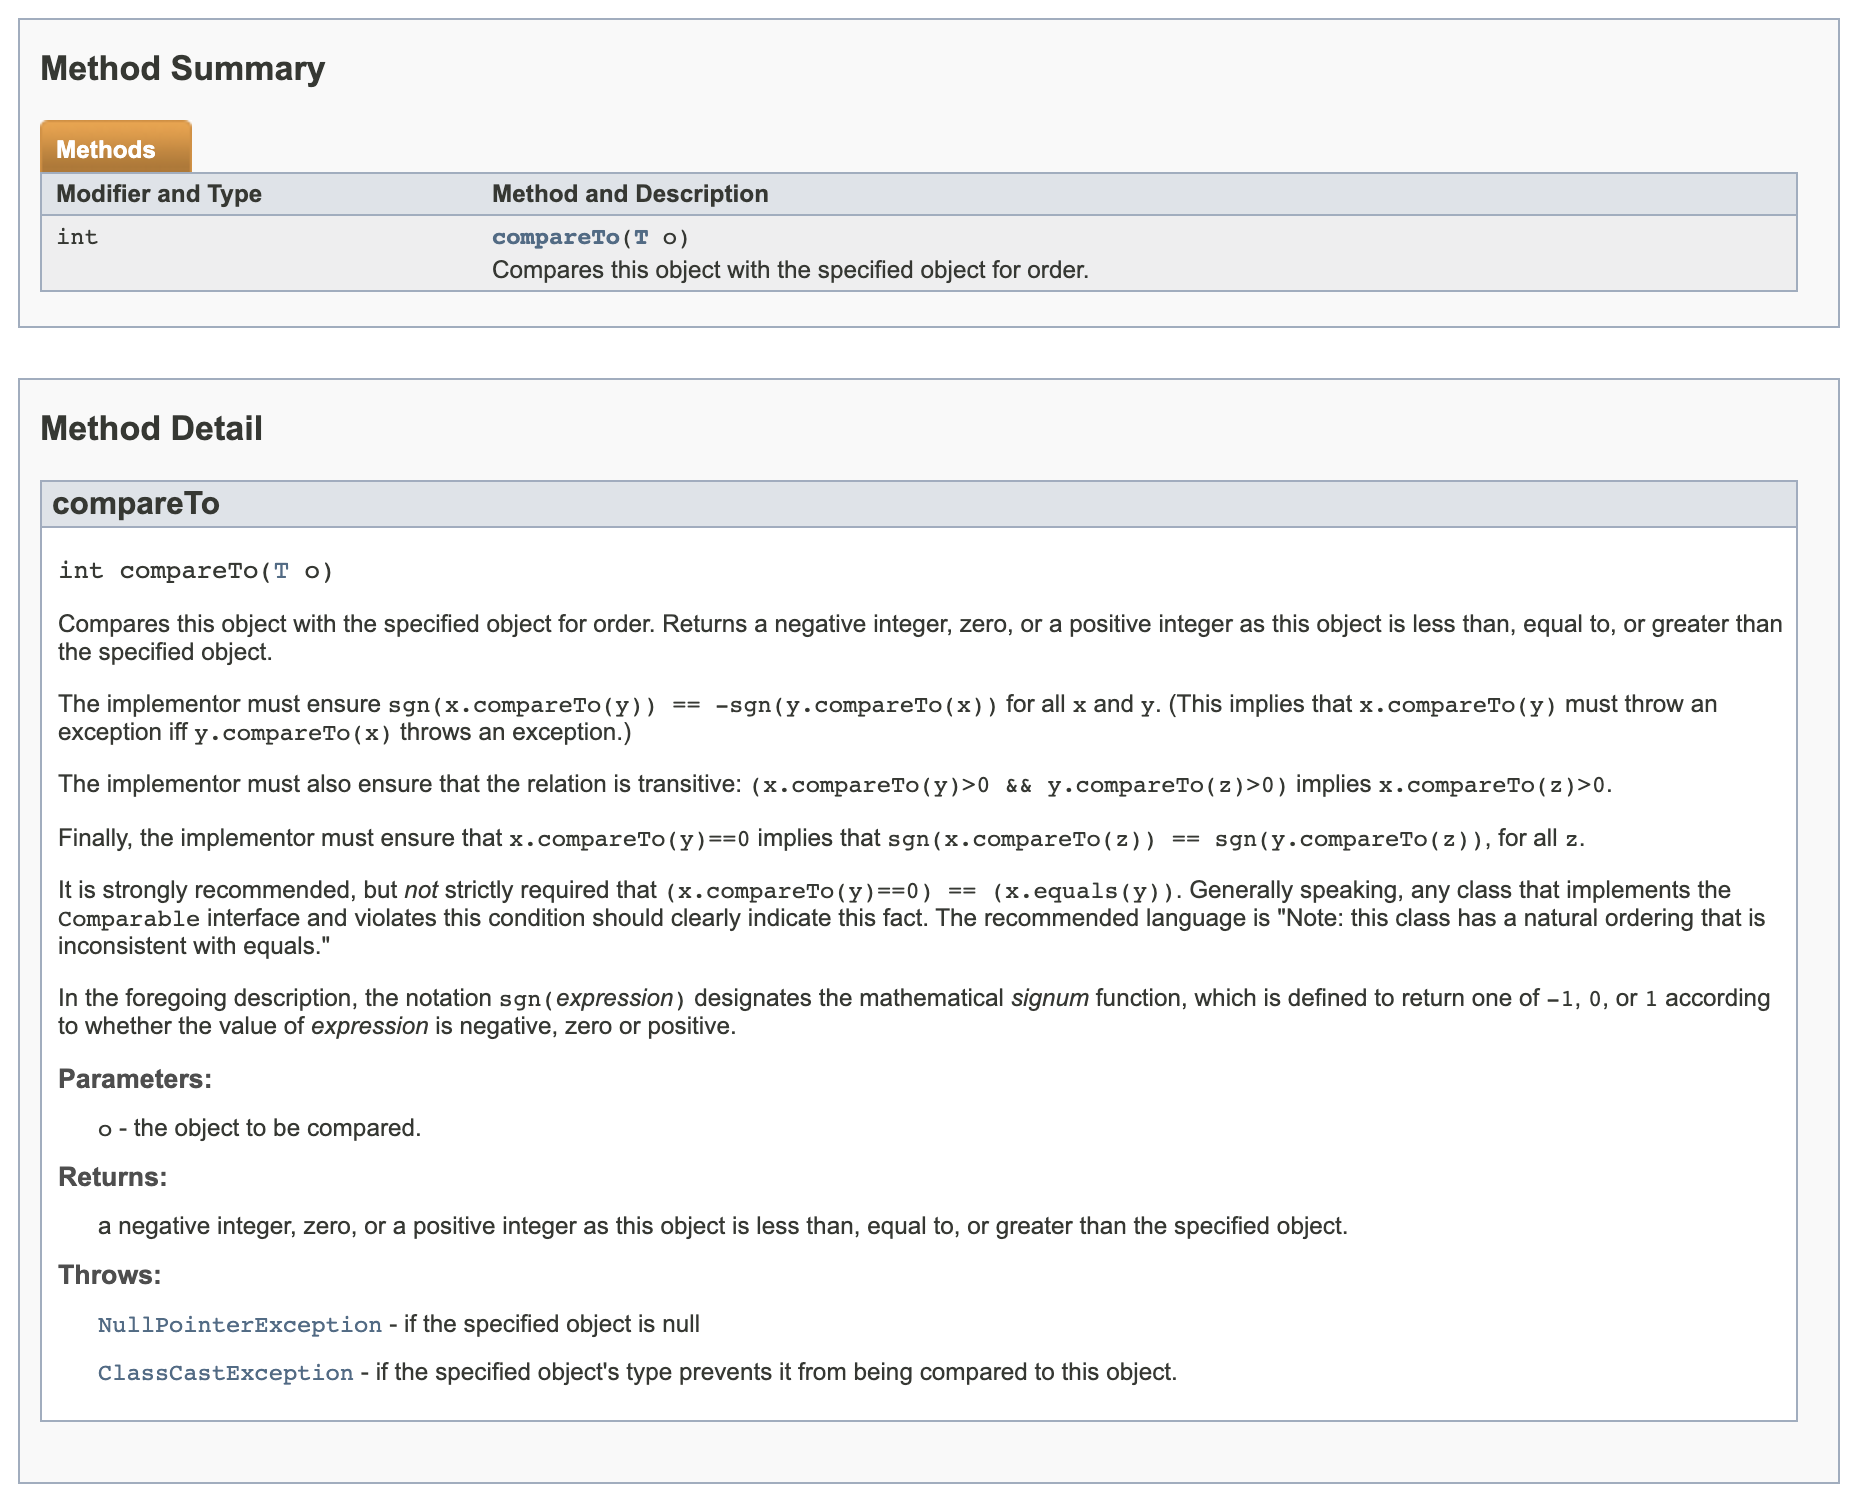
\includegraphics[width=\linewidth]{images/chapter_generics/javadoc_compareTo.png}
\caption{Documentation for interface $Comparable<T>$}
\label{fig:core_classes}
\end{figure}

The class Person has a natural ordering based on the name of a Person-object.  Objects of the class Person can be sorted alphabetically by name. When Person-objects share the same name, we sort by age (younger to older).

\begin{lstlisting}
import java.time.LocalDate;
import java.time.LocalDateTime;
import java.time.temporal.ChronoUnit;
import java.util.Objects;

public class Person implements Comparable<Person> {
	private String name;
	private LocalDate dateOfBirth;

	public Person(String name, LocalDate dateOfBirth) {
		this.name = name;
		this.dateOfBirth = dateOfBirth;
	}

	public int getAge() {
		if (dateOfBirth == null) {
			return 0;
		}
		return (int) ChronoUnit.YEARS.between(dateOfBirth, LocalDateTime.now());
	}
	
	@Override
	public int compareTo(Person other) {
		int nameCompare = this.name.compareTo(other.name);
		if (nameCompare == 0) {
			return other.dateOfBirth.compareTo(this.dateOfBirth);
		}
		return nameCompare;
	}

	public String getName() {
		return name;
	}

	@Override
	public boolean equals(Object o) {
		if (this == o) {
			return true;
		}
		if (o == null || getClass() != o.getClass()) {
			return false;
		}

		Person person = (Person) o;

		if (!Objects.equals(name, person.name)) {
			return false;
		}
		return Objects.equals(dateOfBirth, person.dateOfBirth);
	}

	@Override
	public int hashCode() {
		int result = name != null ? name.hashCode() : 0;
		result = 31 * result + (dateOfBirth != null ? dateOfBirth.hashCode() : 0);
		return result;
	}

	@Override
	public String toString() {
		return "Person{" +
				"name='" + name + '\'' +
				", age='" + getAge() + '\'' +
				'}';
	}
}
\end{lstlisting}

\begin{lstlisting}
package be.pxl.demo;

import java.time.LocalDate;
import java.util.ArrayList;
import java.util.Collections;
import java.util.List;

public class SortingPersons {

	public static void main(String[] args) {
		List<Person> persons = new ArrayList<>();
		Person person1 = new Person("Erik", LocalDate.of(1998, 5, 2));
		Person person2 = new Person("Sam", LocalDate.of(2000, 5, 2));
		Person person3 = new Person("Ann", LocalDate.of(2005, 3, 1));
		Person person4 = new Person("Ann", LocalDate.of(2003, 4, 2));
		Person person5 = new Person("Ann", LocalDate.of(2003, 4, 2));

		persons.add(person1);
		persons.add(person2);
		persons.add(person3);
		persons.add(person4);
		persons.add(person5);

		System.out.println(person3.compareTo(person1));
		System.out.println(person4.compareTo(person3));
		System.out.println(person4.compareTo(person5));

		Collections.sort(persons);
		
		System.out.println(persons);
	}
}
\end{lstlisting}


\begin{verbatim}
-4
2
0
[Person{name='Ann', age='18'}, Person{name='Ann', age='20'}, Person{name='Ann', age='20'}, Person{name='Erik', age='25'}, Person{name='Sam', age='23'}]
\end{verbatim}



\subsection{Writing a generic interface}

Naast generieke klassen kan je ook generieke interfaces en methoden ontwikkelen.
Hier is een voorbeeld van een generieke interface met 2 type-parameters T en U.

\begin{lstlisting}
public interface Service<T,U> {

	T execute(U arg);
}
\end{lstlisting}

Als je beslist om deze interface te implementeren ben je verplicht om de methode execute te implementeren, maar je ben vrij om het datatype voor de parameter en de return-waarde te kiezen.

Hier volgen 2 klassen die de interface Service implementeren.

\begin{lstlisting}
public class CountService implements Service<Integer, String> {

	@Override
	public Integer execute(String arg) {
		return arg.length();
	}
}
\end{lstlisting}

\begin{lstlisting}
import java.util.Random;

public class ProfileService implements Service<Profile, Integer> {

	private static final Random RANDOM = new Random();

  /**
	 * This method can be used to create a Profile-object with a random name and age 18.
	 *
	 * @param length length of the random name of the newly created Profile
	 * @return a newly created Profile-object with a random name of given length and age 18.
	 */
	public Profile execute(Integer length) {
		StringBuilder builder = new StringBuilder();
		for (int i = 0; i < length; i++) {
			int number = RANDOM.nextInt(26) + 97;
			builder.append((char) number);
		}
		Profile profile = new Profile(builder.toString());
		profile.setDateOfBirth(LocalDate.now().minusYears(18));
		return profile;
	}
}
\end{lstlisting}


\begin{lstlisting}
public class GenericServiceDemo {

	public static void main(String[] args) {

		CountService countService = new CountService();
		System.out.println(countService.execute("abcdefghijkl"));

		ProfileService profileService = new ProfileService();
		Profile profile1 = profileService.execute(8);
		System.out.println(profile1);
	}
}
\end{lstlisting}

De uitvoer van bovenstaand programma kan volgende output geven.
\begin{verbatim}
12
Profile{name='tsxjpsol',age=18}
\end{verbatim}


\section{Generieke functies}

Indien je geen nood hebt aan een volledige geparametrizeerde klasse, is het ook mogelijk om geparametrizeerde functies te maken. Zowel gewone als static functies kunnen \'e\'en of meerdere generieke types bevatten. Zelfs een constructor kan gebruikmaken van  generieke types.

Hier volgt een voorbeeld. 
Onderstaande static functie occursExactTimes geeft true indien het opgegeven item het exact opgegeven aantal keren voorkomt in de List. Indien dat niet het geval is, wordt false gegeven.
V\'o\'or het returntype van de functie plaats je eerst een opsomming van de generieke types die gebruikt worden. 
 
\begin{lstlisting}
import java.util.List;

public class OccurenceUtil {

	public static <T> boolean occursExactTimes(List<T> items, T item, int times) {
		int count = 0;
		for (T anItem : items) {
			if (anItem.equals(item)) {
				count++;
			}
		}
		return count == times;
	}

}
\end{lstlisting}

De functie occursExactTimes kan nu gebruikt worden voor elk gewenst datatype.

\begin{lstlisting}
import java.util.Arrays;
import java.util.List;

public class OccurenceUtilDemo {

	public static void main(String[] args) {
		
		List<Integer> numbers = Arrays.asList(7,15,23,12,8,7,23,13,32,7);
		System.out.println(OccurenceUtil.occursExactTimes(numbers, 7, 3));
		System.out.println(OccurenceUtil.occursExactTimes(numbers, 23, 5));

		List<Profile> profiles = Arrays.asList(
				new Profile("Ann"),
				new Profile("Mary"),
				new Profile("Henk"),
				new Profile("Thomas"),
				new Profile("Ann"));
		System.out.println(OccurenceUtil.occursExactTimes(profiles, new Profile("Ann"), 3));
		System.out.println(OccurenceUtil.occursExactTimes(profiles, new Profile("Tommy"), 0));
	}
}
\end{lstlisting}

Bestudeer de code. Welke uitvoer verwacht je?
Komt dat overeen met onze uitvoer? 

\begin{verbatim}
true
false
false
true
\end{verbatim}

\section{Wildcards en bounds}

\subsection{Bounded wildcards}

Bestudeer het volgende programma.

\begin{lstlisting}
import java.util.ArrayList;
import java.util.List;

public class WildcardDemo {


	public static void main(String[] args) {
		List<Movie> movies = new ArrayList<>();
		Movie brotherBear = new Movie("Brother Bear", Rating.LITTLE_KIDS);
		brotherBear.setDuration(125);
		Movie theLionKing = new Movie("The Lion King", Rating.LITTLE_KIDS);
		brotherBear.setDuration(135);
		movies.add(brotherBear);
		movies.add(theLionKing);
		System.out.println(totalDuration(movies));

		List<Documentary> documentaries = new ArrayList<>();
		Documentary planetEarth = new Documentary("Planet Earth", Rating.OLDER_KIDS);
		planetEarth.setDuration(200);
		Documentary ourOcean = new Documentary("Our Ocean", Rating.OLDER_KIDS);
		planetEarth.setDuration(140);
		
		System.out.println(totalDuration(documentaries));
	}


	public static int totalDuration(List<Movie> movies) {
		int totalDuration = 0;
		for (Movie movie: movies) {
			totalDuration += movie.getDuration();
		}
		return totalDuration;
	}
}
\end{lstlisting}

De methode totalDuration kan enkel aangeroepen worden met een List met Movie-objecten. Als je een List met Documentary-objecten hebt zoals in het voorbeeld, zal je een compileerfout krijgen. Eigenlijk is dat zonde. Zou het niet gemakkelijk zijn als de methode totalDuration ook zou werken voor een List met objecten van eender welke subklasse van Movie.

We vervangen nu de signatuur:
\begin{lstlisting}
public static int totalDuration(List<Movie> movies) { ... }
\end{lstlisting}

door: 

\begin{lstlisting}
public static int totalDuration(List<? extends Movie> movies) { ... }
\end{lstlisting}

In deze nieuwe signatuur van de methode totalDuration is een klein maar belangrijk verschil. We hebben het datatype \textit{List$<$Movie$>$} vervangen door \textit{List$<$? extends Movie$>$}. Nu accepteert de methode totalDuration een lijst van eender welke subklasse van Movie, dus kunnen we het ook gebruiken voor $List<Documentary>$. 

We maken hier gebruik van het concept ``bounded wildcard''. Het ? staat voor een nog onbekend datatype, maar we leggen wel grenzen op aan dit onbekende datatype. Zo verplichten we dat dit onbekend datatype de klasse Movie of een subklasse van Movie moet zijn.

In dit voorbeeld had je ook een generieke parameter kunnen gebruiken in plaats van de wildcard, dus \textit{List$<$E extends Movie$>$}.

Je zal af en toe zien dat als  je \'e\'en type parameter gebruikt, je deze kan vervangen door een wildcard. Toch is dat niet altijd waar, kijk maar naar onderstaand voorbeeld waar secondFunction een compileerfout zal geven.
Eigenlijk mag je als vuistregel nemen dat je gegevens met een onbekend datatype (wildcard dus) mag lezen, maar niet mag schrijven.

\begin{lstlisting}
public class Experiment {
    public static <E> void firstFunction(List<E> list) {
        list.add(list.get(0));
    }

    public static void secondFunction(List<?> list) {
        list.add(list.get(0)); // !!!!!!!!!!!!!! won't compile !!!!!!!!!
    }
}
\end{lstlisting}

Er zijn nog enkele verschillen tussen wildcards en type parameters.
Bij type parameters kan je meerdere beperkingen opleggen, bij wildcards niet.

\subsection{Bounds}

Een ``bound'' of grens is een beperking die we opleggen voor de generieke type-parameter. 
Zo zal de methode \textit{void startPlayableContent(T playableContent)} enkel argumenten aanvaarden waarvoor de volgende begrezing geldig is \textit{$<$T extends Content \& Playable$>$}. Dit betekent dat we enkel de klasse Content en zijn subklassen toelaten en ook nog verwachten dat de interface Playable wordt ge\"implementeerd. 
In een begrenzing mag je maximaal 1 klasse opnemen, wat betreft het aantal interfaces is er geen restrictie. De klasse moet wel in de opsomming altijd als eerste staan:
\textit{
$<$T extends MyClass \& MyFirstInterface \& MySecondInterface \& MyThirdInterface$>$}.

\begin{lstlisting}
public class MultipleBoundsDemo {

	public static void main(String[] args) {
		List<Movie> movies = new ArrayList<>();
		Movie brotherBear = new Movie("Brother Bear", Rating.LITTLE_KIDS);
		brotherBear.setDuration(125);
		Movie theLionKing = new Movie("The Lion King", Rating.LITTLE_KIDS);
		brotherBear.setDuration(135);

		List<Documentary> documentaries = new ArrayList<>();
		Documentary planetEarth = new Documentary("Planet Earht", Rating.OLDER_KIDS);
		planetEarth.setDuration(200);
		Documentary ourOcean = new Documentary("Our Ocean", Rating.OLDER_KIDS);
		planetEarth.setDuration(140);

		startPlayableContent(ourOcean);
		startPlayableContent(brotherBear);
	}

	public static <T extends Content & Playable> void startPlayableContent(T playableContent) {
		playableContent.play();
		System.out.println("This content will be playing for " + playableContent.getDuration() + " minutes.");
	}
}
\end{lstlisting}

\subsection{Upper bound, lower bound en unbounded wildcard}

Wanneer je gebruikmaakt van wildcards is het mogelijk om upper bounds (bovengrens) en lower bounds (ondergrens) beperkingen op te leggen. Bij type parameters zijn enkel upper bounds beperkingen mogelijk.

\begin{lstlisting}
import java.util.ArrayList;
import java.util.List;

public class BoundsDemo {

	//Upper bound wildcard
	public static void deleteMovie(List<? extends Movie> movieList, Movie movie) {
		movieList.remove(movie);
	}

	//Lower bound wildcard
	public static void addDocumentary(List<? super Movie> movieList) {
		movieList.add(new Documentary("Hunt for Red October", Rating.OLDER_KIDS));
	}

	//Unbounded wildcard
	public static void printAll(List<?> list) {
		System.out.println("Number of items: " + list.size());
		for (Object item : list) {
			System.out.println(item);
		}
		System.out.println("+++++++++++++++++++++++++++++++");
	}

	public static void main(String[] args) {

		List<Content> contentList = new ArrayList<>();
		List<Movie> movieList = new ArrayList<>();
		List<Documentary> documentaryList = new ArrayList<>();

		addDocumentary(contentList);
		addDocumentary(movieList);
		//addDocumentary(documentaryList);

		printAll(contentList);
		printAll(movieList);

		Movie movie = movieList.get(0);
		deleteMovie(movieList, movie);
		printAll(movieList);
	}

}
\end{lstlisting}

De methode addDocumentary kan gebruikt worden voor $List<Movie>$ maar ook voor iedere superklasse van Movie zoals $List<Content>$ en $List<Object>$.

De methode deleteMovie kan gebruikt worden voor $List<Movie>$ maar ook voor iedere subklasse van Movie zoals $List<Documentary>$.

\begin{oefening}
In het package be.pxl.ja.oefening1 heb je de volgende klassen ter beschikking.

\begin{figure}[H]
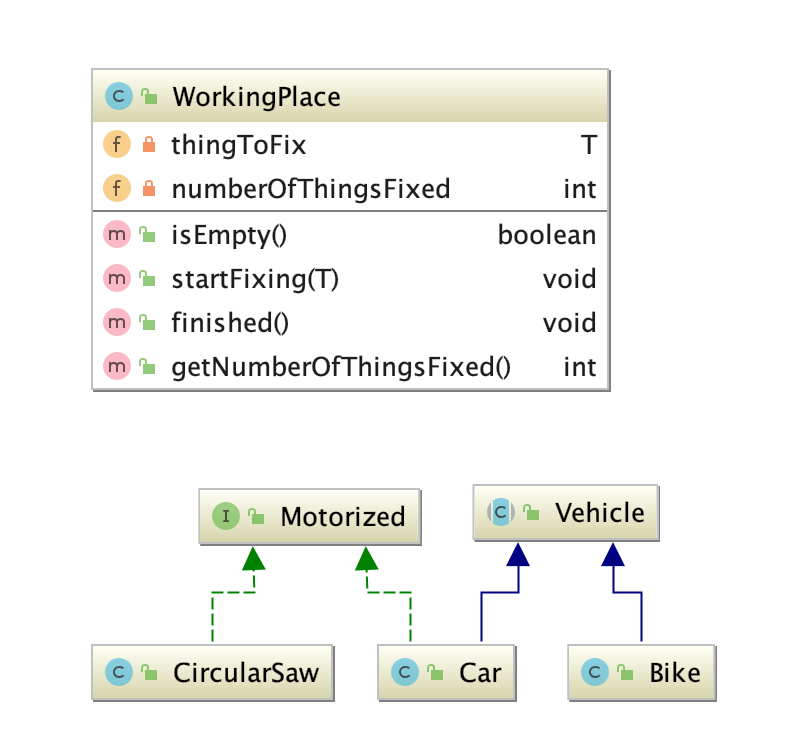
\includegraphics{images/chapter_generics/bounds_exercise_diagram.png}
\caption{Klassenhi\"erarchie}
\label{fig:bounds_exercise}
\end{figure}

\begin{enumerate}[label=(\alph*)]
\item Pas de generieke klasse WorkingPlace aan zodat je WorkingPlace-objecten kan maken om Motorized objecten te herstellen (dus wel WorkingPlace$<$Motorized$>$, WorkingPlace$<$Car$>$, WorkingPlace$<$CircularSaw$>$ maar niet WorkingPlace$<$Bike$>$ of WorkingPlace$<$Vehicle$>$)
\item Pas de generieke klasse WorkingPlace aan zodat je WorkingPlace-objecten kan maken om
Vehicle-objecten te herstellen (dus wel WorkingPlace$<$Car$>$ en WorkingPlace$<$Vehicle$>$).
\item Pas de generieke klasse WorkingPlace aan zodat je WorkingPlace-objecten kan maken om
Motorized-Vehicle-objecten te herstellen.
\end{enumerate}
We passen nu de grenzen van de parameter in de methode getScore in de WorkingPlaceUtility
klasse aan. Test dit telkens uit!
\begin{enumerate}[label=(\alph*)]
\item Zorg ervoor dat je de methode getScore uit WorkingPlaceUtility enkel kan oproepen voor
WorkingPlace$<$Bike$>$-objecten.
\item Zorg ervoor de je de methode getScore uit WorkingPlaceUtility enkel kan oproepen voor
WorkingPlace objecten die Vehicle objecten herstellen.
\item Zorg ervoor de je de methode getScore uit WorkingPlaceUtility enkel kan oproepen voor
WorkingPlace objecten die Motorized objecten herstellen.
\item  Zorg ervoor de je de methode getScore uit WorkingPlaceUtility enkel kan oproepen voor WorkingPlace objecten die Motorized Vehicle objecten herstellen. 
\end{enumerate}
\end{oefening}


\section{Erasure en problemen}

Generics bestaat enkel ``at compiletime''. 
Tijdens het compileren van Java code worden er verschillende extra controles uitgevoerd bij generieke klassen om het correcte gebruik van datatypes te garanderen. 
Vervolgens wordt bij het genereren van de bytecode alle informatie over het generieke datatype gewoon verwijderd. Dus List$<$T$>$ wordt, na enkele controles en toevoegingen van extra code door de compiler, vervangen door List$<$Object$>$ en List$<$T extends Movie$>$ wordt List$<$Movie$>$. Dit noemen we \textbf{type erasure}. In Java zal er dus ook altijd maar \'e\'en gecompileerde klasse (.class-bestand) gegenereerd worden voor een generieke klasse. 

\begin{lstlisting}
List<Integer> list1 = new ArrayList<>();
List<Float> list2 = new ArrayList<>();
if (list1.getClass() == list2.getClass()) {
	System.out.println("Lists have same class.");
}
\end{lstlisting}

Door type erasure is het dus niet mogelijk om generieke static eigenschappen in een klasse te maken.
Ook is het niet mogelijk om een constructor van een generiek datatype aan te roepen.
Daarnaast is het ook niet mogelijk om het generiek datatype te gebruiken bij de operator instanceof.

\begin{lstlisting}
class Box<T> {
   //compiler error
   private static T value;
   private T t;
   
   public Box() {
      // compiler error
   	  t = new T();
   }

   public void set(T t) {
      this.t = t;
   }

   public T get() {
      return t;
   } 
   
   public boolean test() {
	  return t instanceof T;
   }  
}
\end{lstlisting}

\begin{remark}
  Meer weten over generics in java, kijk op pluralsight: \url{https://app.pluralsight.com/player?course=java-generics}. We hebben niet alle onderwerpen die in deze pluralsight cursus aan bod komen gezien.
\end{remark}


\section{Oefening}

\begin{oefening}
Maak een abstract klasse Player met een member variabele name. Voorzie een constructor met name als parameter. 
\\

Maak van deze abstract klasse Player 3 afgeleide klassen: BaseballPlayer, VolleybalPlayer en SoccerPlayer.
\\

Maak nu een klasse Team met de volgende eigenschappen: 
\begin{itemize}
\item name
\item played (=aantal wedstrijden gespeeld)
\item won (= aantal wedstrijden gewonnen)
\item lost (= aantal wedstrijden verloren)
\item tied (=aantal wedstrijden gelijkgespeeld) 
\item members (verzameling van spelers)
\end{itemize}
Voorzie enkel getters. In de constructor geef je  een naam mee voor het team.
\\

Voorzie de methode addPlayer om een speler aan het team toe voegen en een methode
numberOfPlayers om te vragen hoeveel spelers er in het team zitten.
\\

\textbf{Kan je spelers met een verschillend type (bv. BaseballPlayer en SoccerPlayer) in één team
toevoegen? Test uit! Zorg ervoor dat dit niet (meer) mogelijk is.}
\\

Voorzie de methode matchResult(Team opponent, int ourScore, int theirScore). Deze methode zorgt ervoor dat voor het Team waarvoor de methode wordt aangeroepen en de opponent het aantal gespeelde, gewonnen, verloren en gelijkspel wedstrijden wordt opgehoogd afhankelijk van de waarden van ourScore en theirScore.
\\

\textbf{Kan je bovenstaande methode aanroepen voor een team van volleybalspelers tegen een team van baseballspelers? Los dit eventueel op, zodat dat niet langer mogelijk is.}
\\

Voeg tenslotte een methode ranking() toe. Deze geeft een geheel getal terug waarbij het team 3 punten krijgt voor elke gewonnen wedstrijd en 1 punt voor gelijkspel.
Zorg nu dat je een verzameling met Team-objecten kunt aanmaken en deze kunt sorteren op basis van de ranking.
\end{oefening}





Creating a generic class in Java to implement Dijkstra's algorithm for finding the shortest path in a graph is a great way to teach students about generics, graph theory, and algorithms. Here are five use cases for a generic implementation of Dijkstra's algorithm that can be used as programming exercises for your students. These exercises encourage students to apply the algorithm to diverse problems, enhancing their understanding of its versatility and practical applications.

1. Road Network Navigation
Objective: Implement Dijkstra's algorithm to find the shortest path between two locations in a road network. Use the algorithm to calculate the shortest driving distance between cities on a map.

Details: Nodes represent cities, and edges represent roads between cities with distances as weights. Students can use this application to understand how GPS navigation systems suggest the shortest or fastest routes.

2. Network Packet Routing
Objective: Use Dijkstra's algorithm to find the most efficient path for data packets to travel across a computer network from a source to a destination node.

Details: Nodes represent routers or switches in the network, and edges represent the connections between them with latencies as weights. This use case helps students grasp concepts in networking such as routing protocols.

3. Social Networking
Objective: Implement a system that uses Dijkstra's algorithm to find the shortest path of connections between two people in a social network, effectively finding the minimum number of introductions needed to connect two individuals.

Details: Nodes represent users, and edges represent friendships or connections. The weights could represent the strength of connections, helping to understand paths of influence or introduction chains.

4. Resource Distribution Logistics
Objective: Design a system for optimizing the logistics of distributing goods from a warehouse to various delivery points using Dijkstra's algorithm.

Details: Nodes represent distribution centers or delivery points, and edges represent delivery routes with costs or distances as weights. This exercise can demonstrate how logistics companies plan efficient delivery routes.

5. Video Game Pathfinding
Objective: Implement Dijkstra's algorithm for pathfinding in a grid-based video game environment, helping an AI character find the shortest path to a target while avoiding obstacles.

Details: The grid cells are nodes, and edges connect adjacent cells with traversal costs as weights (higher for difficult terrain). This use case introduces students to AI programming concepts and the importance of pathfinding in game development.

Exercise Setup
For each use case, students should:

Design a generic class Graph<T> where T represents the node type. The class should be capable of representing weighted edges between nodes.
Implement Dijkstra's algorithm within the Graph<T> class to find the shortest path between two nodes.
Provide a method to input graph data (nodes and edges), ensuring flexibility to accommodate different types of graphs (directed/undirected, weighted).
Include a method to display the resulting shortest path and its total cost/distance.
Test the implementation with data relevant to the chosen use case to demonstrate the algorithm's application.
These exercises not only cover the implementation of Dijkstra's algorithm in a generic class but also encourage students to think about how algorithms apply to real-world problems across different domains.